\section{Thread Support}

The survey asked different questions about MPI and threads.


Questions 16 (``which MPI features have you never heard of?'') and 17 (``what
aspects of the MPI standard do you use in your program in its current form?'')
reveal that onl 12\% of the respondent (86/692) have never heard about
MPI+OpenMP or multithreading and that 58\% of the respondents are using
multithreading or OpenMP in their program.


Question 18 was about the thread support that is used in the MPI applications
of the respondent.  

\begin{table}[htb]%
\begin{center}%
\caption{Q18: Which MPI thread support are you using?}%
\label{tab:Q18-ans}%
\begin{tabular}{l|l|r}%
\hline%
Choice & Abbrv. & \# Answers \\%
\hline%
MPI\_THREAD\_SINGLE & SINGLE & 238 (28.7\%) \\%
MPI\_THREAD\_FUNNELED & FUNNELED & 145 (17.5\%) \\%
MPI\_THREAD\_SERIALIZED & SERIALIZED & 99 (11.9\%) \\%
MPI\_THREAD\_MULTIPLE & MULTIPLE & 261 (31.4\%) \\%
I have never called MPI\_INIT\_THREAD & never used & 267 (32.2\%) \\%
I do not know or I do not care. & do not know/care & 168 (20.2\%) \\%
\hline%
\multicolumn{2}{c}{total} & 1178 (830)\\%
\hline%
\end{tabular}%
\end{center}%
\end{table}%


The support of multi-threading in MPI is done in different ways (MPI\_THREAD\_SINGLE
MPI\_THREAD\_FUNNELED, MPI\_THREAD\_SERIALIZED, MPI\_THREAD\_MULTIPLE, in order of
decreasing semantic restriction and often decreasing performance). The most used options (42.5\%) are either
MPI\_THREAD\_SINGLE or MPI\_THREAD\_MULTIPLE which are the at the two ends of the
spectrum in terms of thread support. This means that  most users either want a full support or a
limited support. This could also mean that intermediate thread support which can
offer a different trade-off between performance and semantic, requires more effort to be
implemented efficiently within a program. Moreover, almost 37.1\% of the answers
show no usage of thread
support in their program. Region-wise (see Fig.~\ref{fig:Q18}), we see that in the USA, thread support is more used
than in other regions and the most used option is MPI\_THREAD\_MULTIPLE which is
the least restrictive option. 

\begin{figure}[htb]
\begin{center}
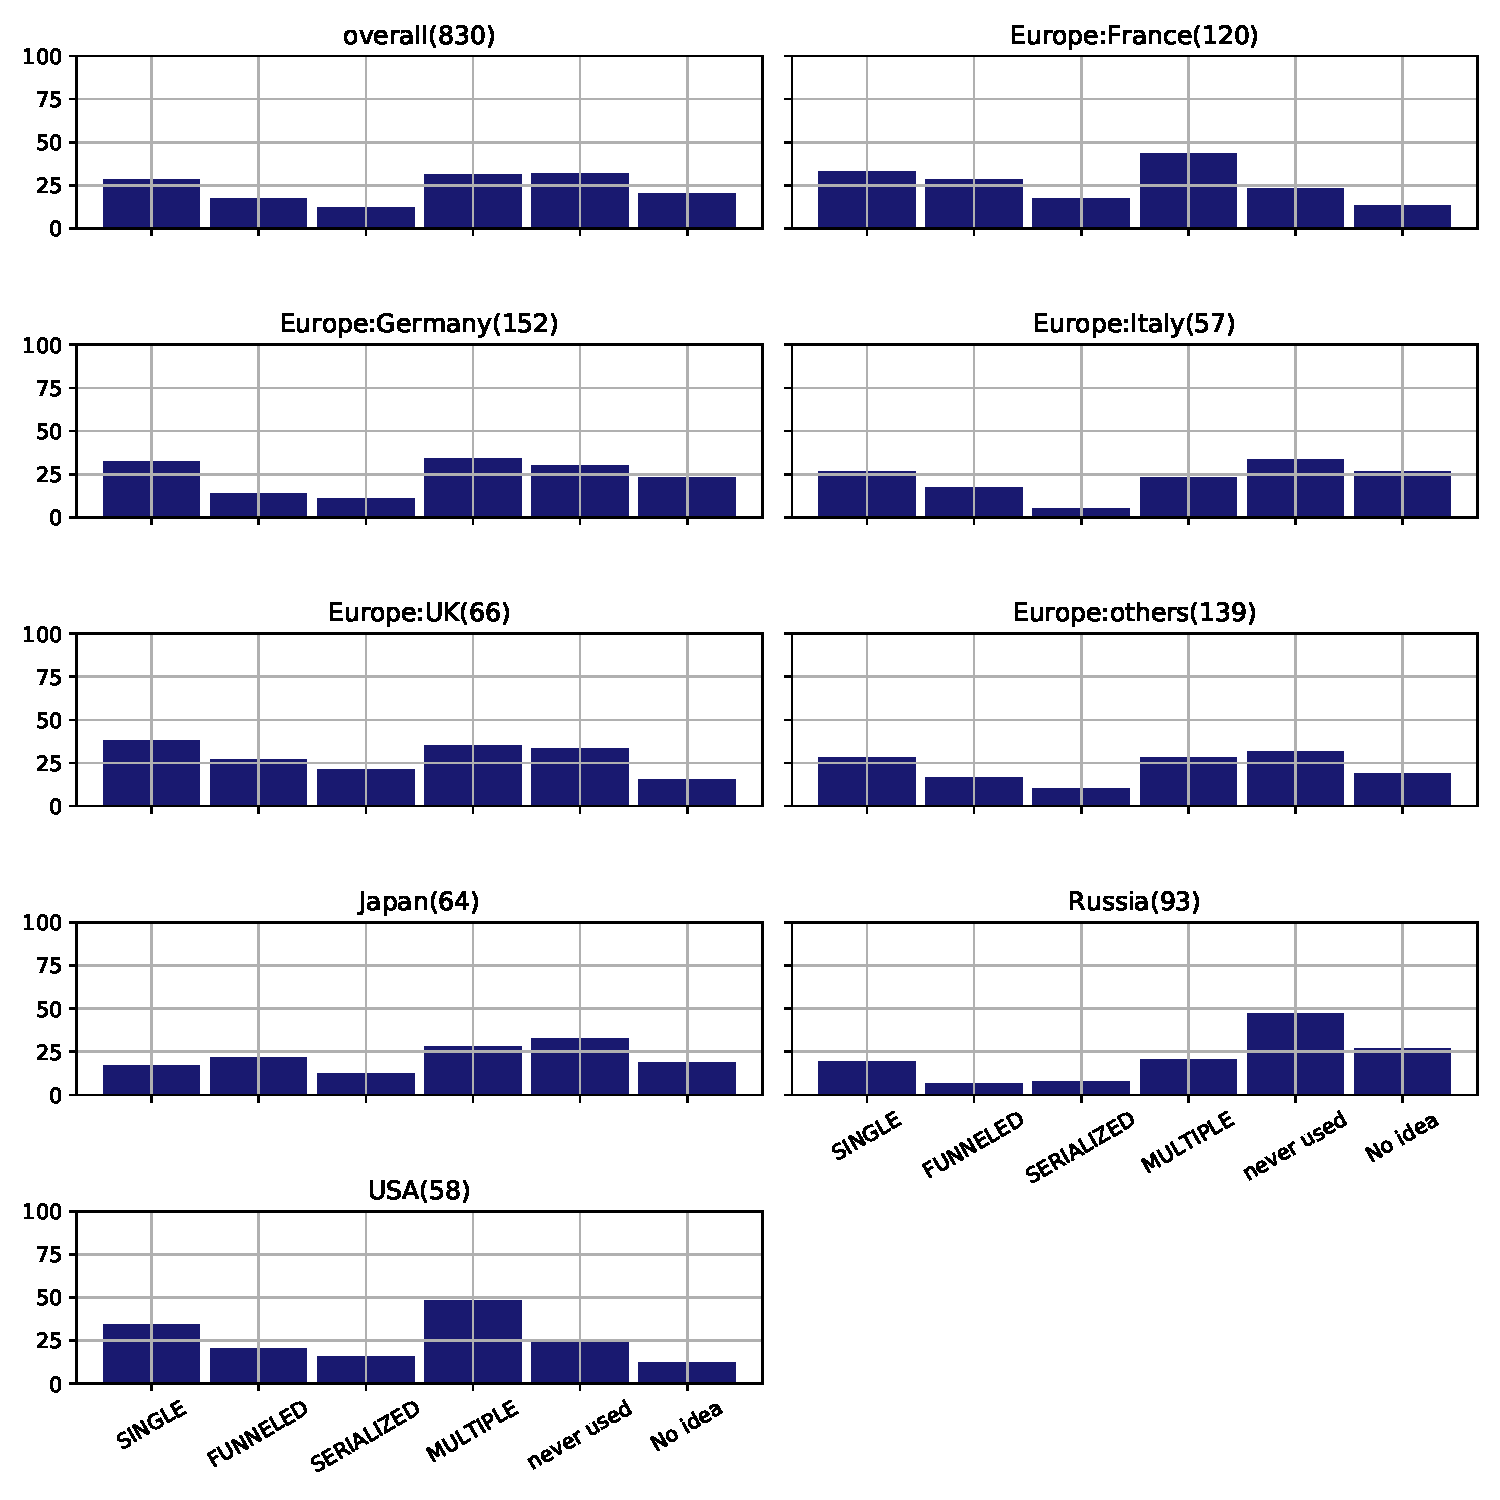
\includegraphics[width=10cm]{../pdfs/Q18.pdf}
\caption{Simple analysis: Q18}
\label{fig:Q18}
\end{center}
\end{figure}


However, this question is a multi-answer question. We can see the distribution
of the different answers among the respondent in Table~\ref{tab:Q18-mans}. If we
remove inconsistent answers (such as ``SINGLE'' and ``Never used'') we  have 806
consitent responders. Among them, the 
number of participants who answered ``I have never called
MPI\_INIT\_THREAD'' or ``I do not know or I do not care'' dominates
close to 49\% (394/806).  In the rest of the half, the
number of specifying one of the thread level and the number of
specifying two or more of them are comparable. 


\clearpage%
{\footnotesize\begin{landscape}%
\begin{longtable}[htb]{r|c|c|c|c|c|c|c|c|c|c}%
\caption{Q18: Which MPI thread support are you using?}%
\label{tab:Q18-mans} \\%
\hline%
Multi-Answer & overall & FR & GR & IT & UK & eu & JP & RU & US & others \\
 \hline%
\endfirsthead%
\multicolumn{11}{r}{(continued from the previous page)}\\%
\hline%
Multi-Answer & overall & FR & GR & IT & UK & eu & JP & RU & US & others \\
 \hline%
\endhead%
\hline%
(total) & 830 & 120 & 152 & 57 & 66 & 139 & 64 & 93 & 58 & 81 \\%
\hline%
\multicolumn{11}{r}{(continue to the next page)}\\%
\endfoot%
\hline%
(total) & 830 & 120 & 152 & 57 & 66 & 139 & 64 & 93 & 58 & 81 \\%
\hline%
\endlastfoot%
\hline%
{never used} & 234 & 24 & 40 & 15 & 20 & 40 & 19 & 39 & 14 & 23 \\%
{No idea} & 143 & 14 & 29 & 13 & 8 & 25 & 11 & 20 & 5 & 18 \\%
{MULTIPLE} & 97 & 18 & 19 & 7 & 7 & 15 & 9 & 5 & 8 & 9 \\%
{SINGLE, MULTIPLE} & 70 & 11 & 17 & 3 & 4 & 13 & 2 & 9 & 6 & 5 \\%
{SINGLE} & 59 & 7 & 12 & 6 & 5 & 11 & 1 & 2 & 5 & 10 \\%
{FUNNELED} & 36 & 5 & 4 & 5 & 1 & 11 & 4 & 3 & 1 & 2 \\%
{SINGLE, FUNNELED, SERIALIZED, MULTIPLE} & 34 & 9 & 9 & 2 & 8 & 1 & 1 & 0 & 3 & 1 \\%
{SINGLE, FUNNELED} & 28 & 8 & 7 & 1 & 3 & 3 & 3 & 1 & 0 & 2 \\%
{never used, No idea} & 23 & 2 & 6 & 2 & 2 & 1 & 1 & 5 & 1 & 3 \\%
{SERIALIZED} & 23 & 5 & 1 & 0 & 1 & 3 & 4 & 2 & 4 & 3 \\%
{FUNNELED, MULTIPLE} & 18 & 7 & 0 & 0 & 0 & 1 & 4 & 0 & 5 & 1 \\%
{SINGLE, FUNNELED, MULTIPLE} & 12 & 1 & 1 & 0 & 2 & 2 & 1 & 2 & 3 & 0 \\%
{SINGLE, SERIALIZED, MULTIPLE} & 10 & 1 & 2 & 0 & 0 & 3 & 0 & 2 & 2 & 0 \\%
{SERIALIZED, MULTIPLE} & 10 & 1 & 4 & 0 & 1 & 2 & 1 & 1 & 0 & 0 \\%
{SINGLE, FUNNELED, SERIALIZED} & 9 & 0 & 0 & 1 & 3 & 3 & 1 & 0 & 0 & 1 \\%
{SINGLE, SERIALIZED} & 7 & 1 & 1 & 0 & 0 & 1 & 1 & 2 & 0 & 1 \\%
{FUNNELED, SERIALIZED, MULTIPLE} & 5 & 3 & 0 & 0 & 1 & 1 & 0 & 0 & 0 & 0 \\%
{SINGLE, never used} & 5 & 1 & 0 & 1 & 0 & 1 & 1 & 0 & 0 & 1 \\%
{SINGLE, MULTIPLE, never used} & 2 & 1 & 0 & 0 & 0 & 1 & 0 & 0 & 0 & 0 \\%
{SINGLE, FUNNELED, MULTIPLE, never used} & 1 & 0 & 0 & 1 & 0 & 0 & 0 & 0 & 0 & 0 \\%
{FUNNELED, never used} & 1 & 0 & 0 & 0 & 0 & 1 & 0 & 0 & 0 & 0 \\%
{MULTIPLE, never used, No idea} & 1 & 0 & 0 & 0 & 0 & 0 & 0 & 0 & 0 & 1 \\%
{SINGLE, MULTIPLE, No idea} & 1 & 0 & 0 & 0 & 0 & 0 & 0 & 0 & 1 & 0 \\%
{FUNNELED, SERIALIZED} & 1 & 1 & 0 & 0 & 0 & 0 & 0 & 0 & 0 & 0 \\%
\hline%
\end{longtable}%
\end{landscape}}%
\clearpage%



Another question is related to hybrid programming (Q22 : Have you ever written
MPI+X programs?).  This is also a mutli-answer question related to hybrid
programming which often involves threading (e.g. OpenMP). 

\begin{table}[htb]%
\begin{center}%
\caption{Q22: Have you ever written MPI+”X” programs? If so, select all that apply.}%
\label{tab:Q22-ans}%
\begin{tabular}{l|l|r}%
\hline%
Choice & Abbrv. & \# Answers \\%
\hline%
OpenMP & OMP & 577 (69.7\%) \\%
CUDA & CUDA & 231 (27.9\%) \\%
No & No & 190 (22.9\%) \\%
Pthread & Pthread & 155 (18.7\%) \\%
OpenACC & OACC & 79 (9.5\%) \\%
OpenCL & OCL & 43 (5.2\%) \\%
other & - & 33 (4.0\%) \\%
\hline%
\multicolumn{2}{c}{total} & 1308 (828)\\%
\hline%
\end{tabular}%
\end{center}%
\end{table}%



According to table~\ref{tab:q22-ans} only a small fraction (15\%) of the usage
of  MPI do not imply  any other parallel programming language/model. The language
or API the most used with MPI is OpenMP (44\%) followed by CUDA
(17\%). As it is a multi-answer question, we see from table~\ref{tab:q22-mans}
that  only 23\% (190/815) of the respondents have never written an MPI program
without any other programming language or model. 

\clearpage%
{\footnotesize\begin{landscape}%
\begin{longtable}[htb]{r|c|c|c|c|c|c|c|c|c|c}%
\caption{Q22: Have you ever written MPI+”X” programs? If so, select all that apply.}%
\label{tab:Q22-mans} \\%
\hline%
Multi-Answer & overall & FR & GR & IT & UK & eu & JP & RU & US & others \\
 \hline%
\endfirsthead%
\multicolumn{11}{r}{(continued from the previous page)}\\%
\hline%
Multi-Answer & overall & FR & GR & IT & UK & eu & JP & RU & US & others \\
 \hline%
\endhead%
\hline%
(total) & 828 & 119 & 156 & 54 & 65 & 140 & 64 & 91 & 57 & 82 \\%
\hline%
\multicolumn{11}{r}{(continue to the next page)}\\%
\endfoot%
\hline%
(total) & 828 & 119 & 156 & 54 & 65 & 140 & 64 & 91 & 57 & 82 \\%
\hline%
\endlastfoot%
\hline%
{OMP} & 270 & 37 & 62 & 19 & 22 & 43 & 25 & 27 & 14 & 21 \\%
{No} & 190 & 24 & 41 & 19 & 13 & 28 & 8 & 25 & 5 & 27 \\%
{OMP, CUDA} & 94 & 4 & 9 & 9 & 6 & 22 & 7 & 18 & 9 & 10 \\%
{OMP, Pthread} & 60 & 14 & 13 & 1 & 11 & 7 & 4 & 2 & 5 & 3 \\%
{OMP, Pthread, CUDA} & 36 & 5 & 9 & 0 & 1 & 4 & 4 & 4 & 6 & 3 \\%
{OMP, OACC} & 24 & 6 & 2 & 1 & 2 & 7 & 3 & 0 & 0 & 3 \\%
{OMP, OACC, CUDA} & 21 & 3 & 4 & 0 & 1 & 3 & 4 & 0 & 3 & 3 \\%
{CUDA} & 19 & 1 & 0 & 0 & 2 & 4 & 2 & 5 & 3 & 2 \\%
{Pthread} & 16 & 4 & 0 & 1 & 2 & 2 & 0 & 3 & 3 & 1 \\%
{OMP, OCL, CUDA} & 14 & 4 & 0 & 1 & 0 & 5 & 0 & 2 & 2 & 0 \\%
{OMP, Pthread, OACC, CUDA} & 9 & 1 & 1 & 0 & 1 & 0 & 3 & 0 & 1 & 2 \\%
{OMP, Pthread, OCL, CUDA} & 7 & 1 & 2 & 1 & 0 & 1 & 0 & 0 & 1 & 1 \\%
{OMP, OACC, OCL, CUDA} & 5 & 0 & 1 & 1 & 0 & 2 & 0 & 0 & 1 & 0 \\%
{Pthread, CUDA} & 5 & 2 & 0 & 0 & 0 & 2 & 0 & 1 & 0 & 0 \\%
{OMP, Pthread, OACC, OCL, CUDA} & 4 & 0 & 1 & 1 & 0 & 1 & 1 & 0 & 0 & 0 \\%
{OMP, Pthread, OACC} & 3 & 0 & 1 & 0 & 1 & 0 & 1 & 0 & 0 & 0 \\%
{OCL} & 3 & 1 & 0 & 0 & 0 & 0 & 0 & 1 & 0 & 1 \\%
{Pthread, OACC} & 2 & 1 & 0 & 0 & 0 & 0 & 0 & 0 & 0 & 1 \\%
{OMP, TBB} & 2 & 0 & 1 & 0 & 0 & 0 & 0 & 0 & 1 & 0 \\%
{Pthread, OCL, CUDA} & 2 & 0 & 0 & 0 & 0 & 1 & 0 & 1 & 0 & 0 \\%
{OACC} & 2 & 0 & 0 & 0 & 1 & 1 & 0 & 0 & 0 & 0 \\%
{OACC, CUDA} & 2 & 1 & 0 & 0 & 0 & 1 & 0 & 0 & 0 & 0 \\%
{OMP, OACC, OCL} & 2 & 0 & 1 & 0 & 0 & 0 & 0 & 0 & 1 & 0 \\%
{OMP, GASPI} & 2 & 0 & 2 & 0 & 0 & 0 & 0 & 0 & 0 & 0 \\%
{OCL, CUDA} & 2 & 1 & 0 & 0 & 0 & 1 & 0 & 0 & 0 & 0 \\%
{OMP, Pthread, OCL} & 2 & 2 & 0 & 0 & 0 & 0 & 0 & 0 & 0 & 0 \\%
{OMP, Pthread, Cilk++} & 1 & 1 & 0 & 0 & 0 & 0 & 0 & 0 & 0 & 0 \\%
{OMP, coupling applications implemented in various languages (C++, fortran, Python) with MPI} & 1 & 1 & 0 & 0 & 0 & 0 & 0 & 0 & 0 & 0 \\%
{OMP, MPI-3 shared memory windows} & 1 & 0 & 1 & 0 & 0 & 0 & 0 & 0 & 0 & 0 \\%
{OMP, CUDA, Python} & 1 & 0 & 0 & 0 & 0 & 0 & 0 & 1 & 0 & 0 \\%
{OMP, Pthread, StarPU} & 1 & 1 & 0 & 0 & 0 & 0 & 0 & 0 & 0 & 0 \\%
{OMP, Pthread, OACC, CUDA, TBB, C++11 threads.} & 1 & 0 & 0 & 0 & 0 & 1 & 0 & 0 & 0 & 0 \\%
{CUDA, StarPU, Intel TBB, MassiveThreads} & 1 & 0 & 0 & 0 & 0 & 0 & 1 & 0 & 0 & 0 \\%
{OMP, Pthread, MPI + Pthread but only via library (PaStiX)} & 1 & 0 & 1 & 0 & 0 & 0 & 0 & 0 & 0 & 0 \\%
{Sunway athread} & 1 & 0 & 0 & 0 & 0 & 0 & 0 & 0 & 0 & 1 \\%
{OMP, Pthread, OCL, CUDA, C++ threads} & 1 & 0 & 0 & 0 & 0 & 1 & 0 & 0 & 0 & 0 \\%
{OMP, OACC, TBB} & 1 & 0 & 0 & 0 & 1 & 0 & 0 & 0 & 0 & 0 \\%
{OMP, Pthread, OmpSs} & 1 & 0 & 1 & 0 & 0 & 0 & 0 & 0 & 0 & 0 \\%
{OMP, CUDA, MPI + MPI} & 1 & 0 & 0 & 0 & 1 & 0 & 0 & 0 & 0 & 0 \\%
{OMP, tbb GASPI} & 1 & 1 & 0 & 0 & 0 & 0 & 0 & 0 & 0 & 0 \\%
{OMP, CUDA, kokkos} & 1 & 1 & 0 & 0 & 0 & 0 & 0 & 0 & 0 & 0 \\%
{OMP, Pthread, CUDA, Tbb} & 1 & 1 & 0 & 0 & 0 & 0 & 0 & 0 & 0 & 0 \\%
{Julia GPU} & 1 & 0 & 0 & 0 & 0 & 0 & 0 & 0 & 1 & 0 \\%
{OMP, OACC, ompss} & 1 & 1 & 0 & 0 & 0 & 0 & 0 & 0 & 0 & 0 \\%
{Pthread, UPC, UPC++} & 1 & 0 & 0 & 0 & 0 & 0 & 0 & 0 & 1 & 0 \\%
{Sunway Athread, OACC} & 1 & 0 & 0 & 0 & 0 & 0 & 0 & 0 & 0 & 1 \\%
{OMP, OCL} & 1 & 0 & 1 & 0 & 0 & 0 & 0 & 0 & 0 & 0 \\%
{athread} & 1 & 0 & 0 & 0 & 0 & 0 & 0 & 0 & 0 & 1 \\%
{OMP, CUDA, Intel TBB} & 1 & 0 & 1 & 0 & 0 & 0 & 0 & 0 & 0 & 0 \\%
{Pthread, TensorFlow} & 1 & 0 & 0 & 0 & 0 & 0 & 1 & 0 & 0 & 0 \\%
{OMP, Just as exercise in classes, or seen in others' programs} & 1 & 0 & 0 & 0 & 0 & 1 & 0 & 0 & 0 & 0 \\%
{OMP, OACC, CUDA, CUDA Fortran} & 1 & 0 & 0 & 0 & 0 & 1 & 0 & 0 & 0 & 0 \\%
{OMP, Kokkos} & 1 & 0 & 0 & 0 & 0 & 0 & 0 & 0 & 0 & 1 \\%
{OMP, ("MPI + MPI-3 shared memory" instead of "MPI+OpenMP")} & 1 & 0 & 1 & 0 & 0 & 0 & 0 & 0 & 0 & 0 \\%
{CUDA, Posix ShM} & 1 & 0 & 0 & 0 & 0 & 0 & 0 & 1 & 0 & 0 \\%
{OMP, CUDA, ROCm} & 1 & 0 & 0 & 0 & 0 & 1 & 0 & 0 & 0 & 0 \\%
\hline%
\end{longtable}%
\end{landscape}}%
\clearpage%


Related to thread support for computing (not taking into account CUDA or
OpenCL which mostly use thread at the MPI level for managing data), we see that a
majority of the usages (OpenMP, Pthread, etc.)  implies threading at some point.


\begin{figure}[htb]
\begin{center}
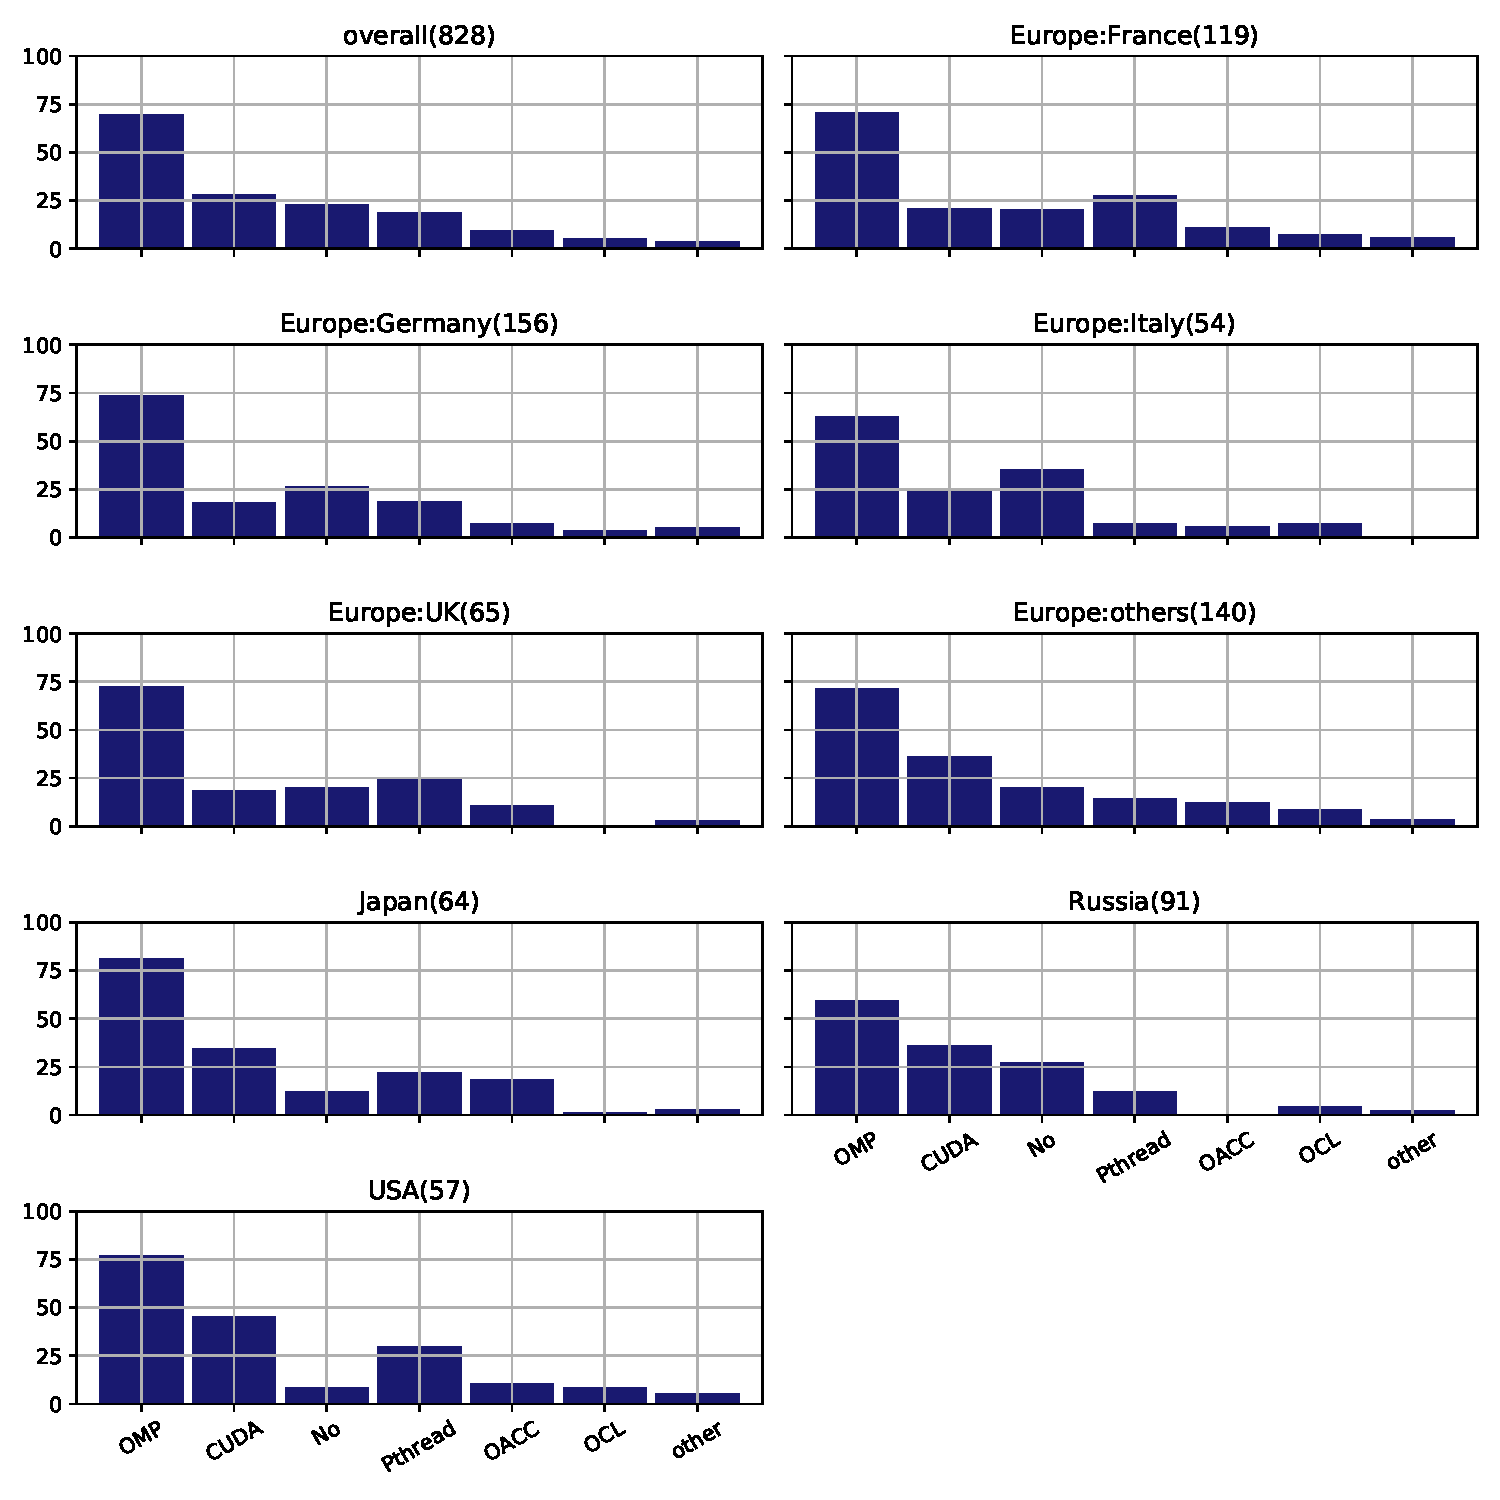
\includegraphics[width=10cm]{../pdfs/Q22.pdf}
\caption{Simple analysis: Q22}
\label{fig:Q22}
\end{center}
\end{figure}

If we look at the answers in terms of region (fig~\ref{fig:Q22}), we see that In
general, around 40\% of all countries/regions exhibit an MPI usage with OpenMP. The
hybrid technique is very common.  It is interesting that the percentage of 'no'
answer in the US is the smallest.

In conclusion, it appears that in the majority of the cases, MPI and threads are
often used conjointly.  This is not very surprising as, with the advent of
multi-core nodes, many programs use less MPI processes than cores and these
processes are then multithreaded. Hence, due to this importance it is necessary
that MPI continue and extend its support to multithreaded and hybrid programming.